\chapter{Model Training and Optimization}
\label{ch:chapter06}
 
%
% Section: 6 - Intro
%

\ac{BERT}, specifically \ac{Sci-BERT}, multi-class classifier model has been trained and tested using \ac{SoMeSci} data set. The model has been trained in various training scenarios to determine conditions that leads to improved performance of classifier. The training scenarios considered, the effect of context information  and the impact of including or excluding parts of \ac{SoMeSci} data set on the classifier’s performance.\\
 
Furthermore, software purpose classifier’s performance has also been investigated by removing mention-type and software-type classifiers from cascades of classifier modules.  In addition, the impact of using another variant of BERT model, \ac{Bio-BERT}, on classifier’s performance  has also been investigated. \\

Finally, results from all training scenarios have been discussed and best performing model has been selected based on the results of investigation.

\section{The impact of labeled data}
\label{sec:chapter06:exclusion}

As described in the table 4.1 before, the \ac{SoMeSci} dataset is composed of 4 different sets of articles: \emph{PLoS-methods, PubMed-full text,  PLoS-sentences} and \emph{creation-sentences}. Since only articles in the  \emph{PLoS-methods} and \emph{PubMed-full text} are annotated with software usage purpose labels, it was desired to evaluate weather including \emph{PLoS} and \emph{Creation}, which are not labeled with software usage purpose, would result in improved performance of the software usage purpose classifier.  \\

The results of evaluation indicates that including \emph{ PLoS-sentences} and \emph{creation-sentences} in the training dataset, definitely improved the overall performance for classification of software, but not for software usage purpose. Figure 6.1 below shows total F-score for software classification over test and development data sets is increased with the inclusion of \emph{PLoS/Creation} sentences in the data set. \\

\begin{figure}[htbp]
	\centering
	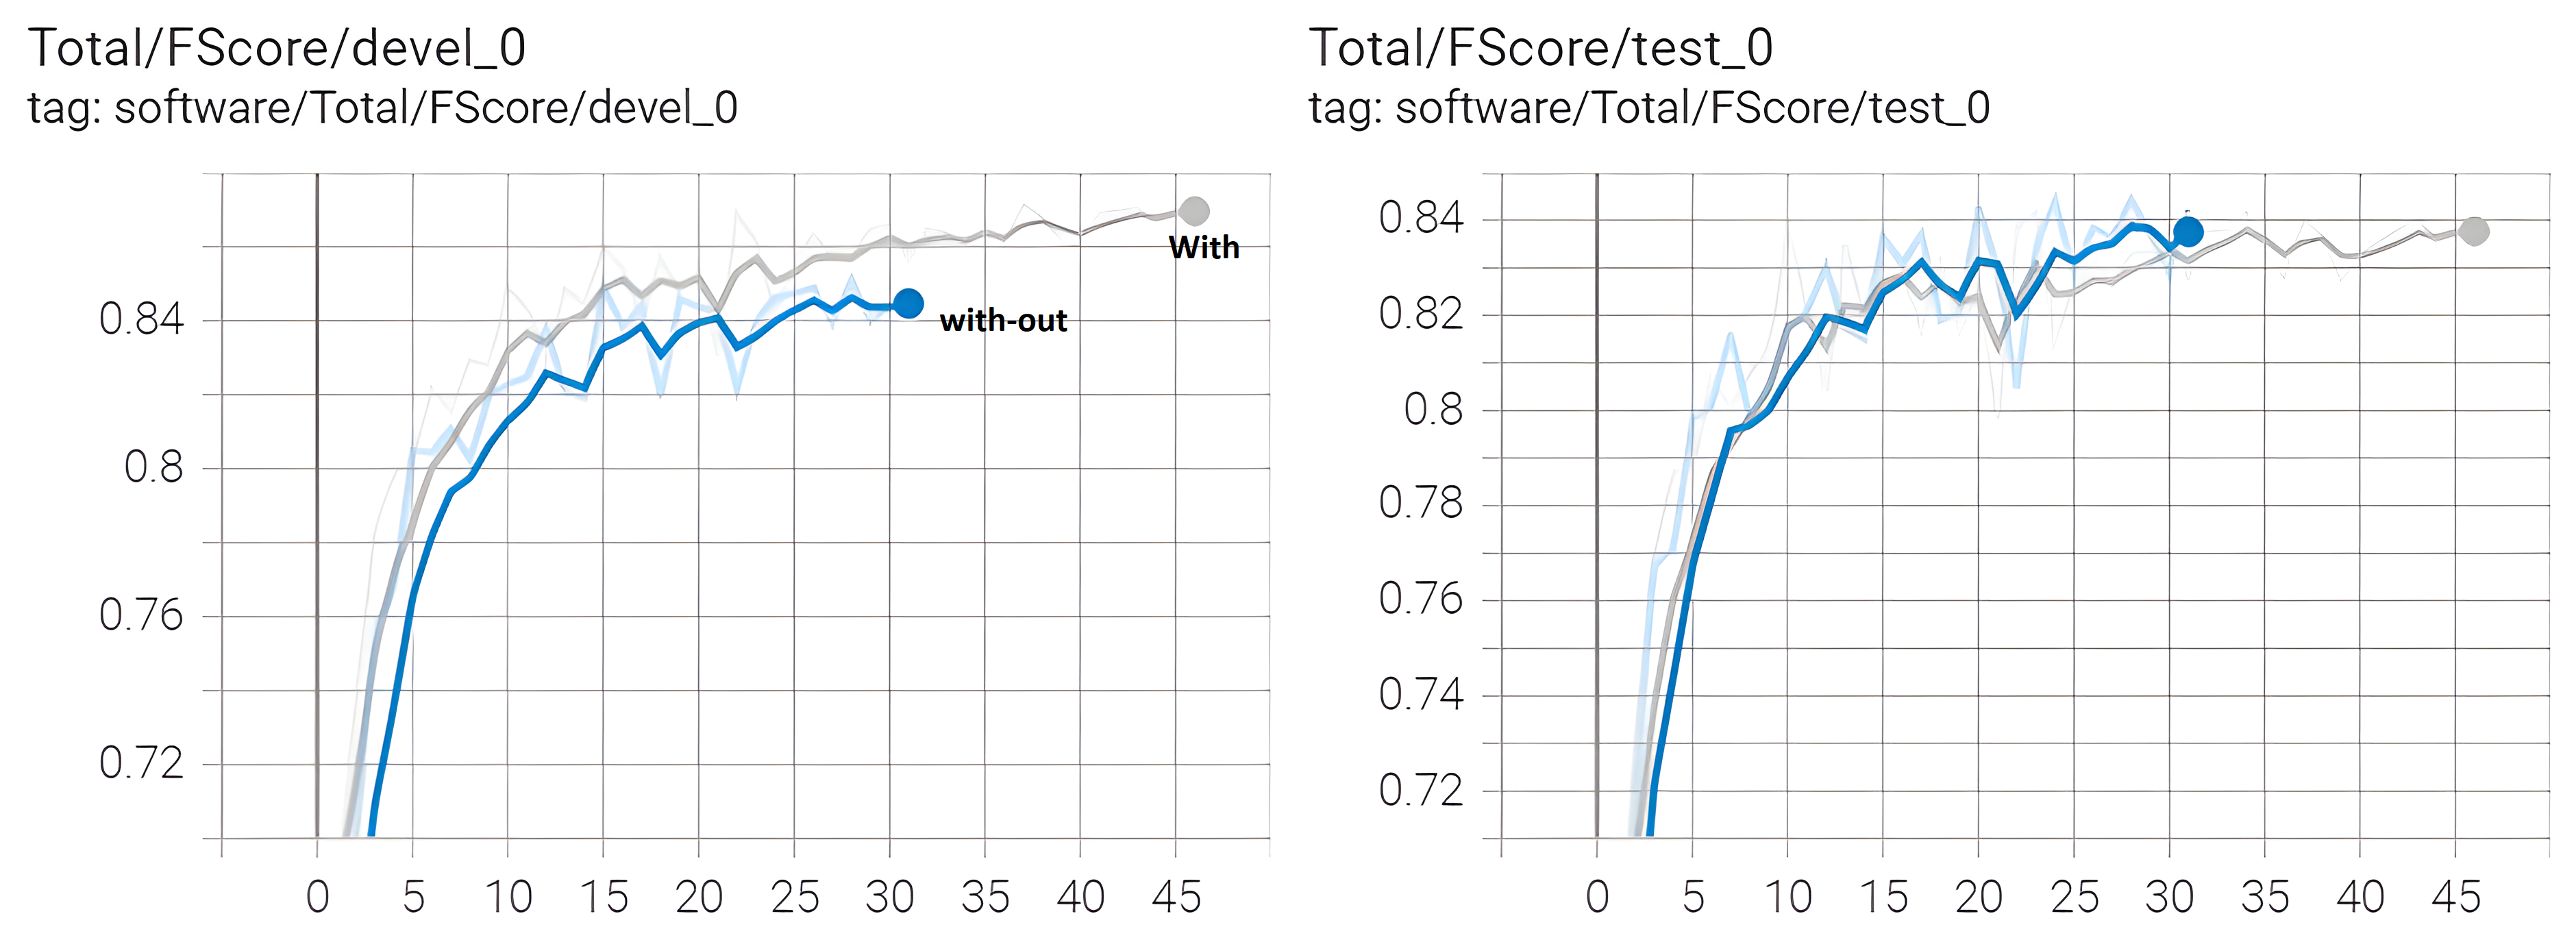
\includegraphics[width=.86\textwidth]{4.graphics/figures/ch_6/1.with_sent_vs_without/HD/TotalFscoresoftware}
	\caption{Software classification (Total) F1-score for devel (left) and test(right) shows improvement when \emph{Creation/PLoS} sentences are included in the training dataset.}
	\label{fig:chapter06:with}
\end{figure}


In contrast, the overall performance of the software purpose classifier is diminished when trained with \emph{ PLoS-sentences} and \emph{creation-sentences} in addition to \emph{ PLoS-methods}, \emph{PubMed-full text}. Figure 6.2 below depicts, Fscore for software purpose classifier is deteriorated when trained along with \emph{Creation/PLoS} sentences.  \\

\begin{figure}[htbp]
	\centering
	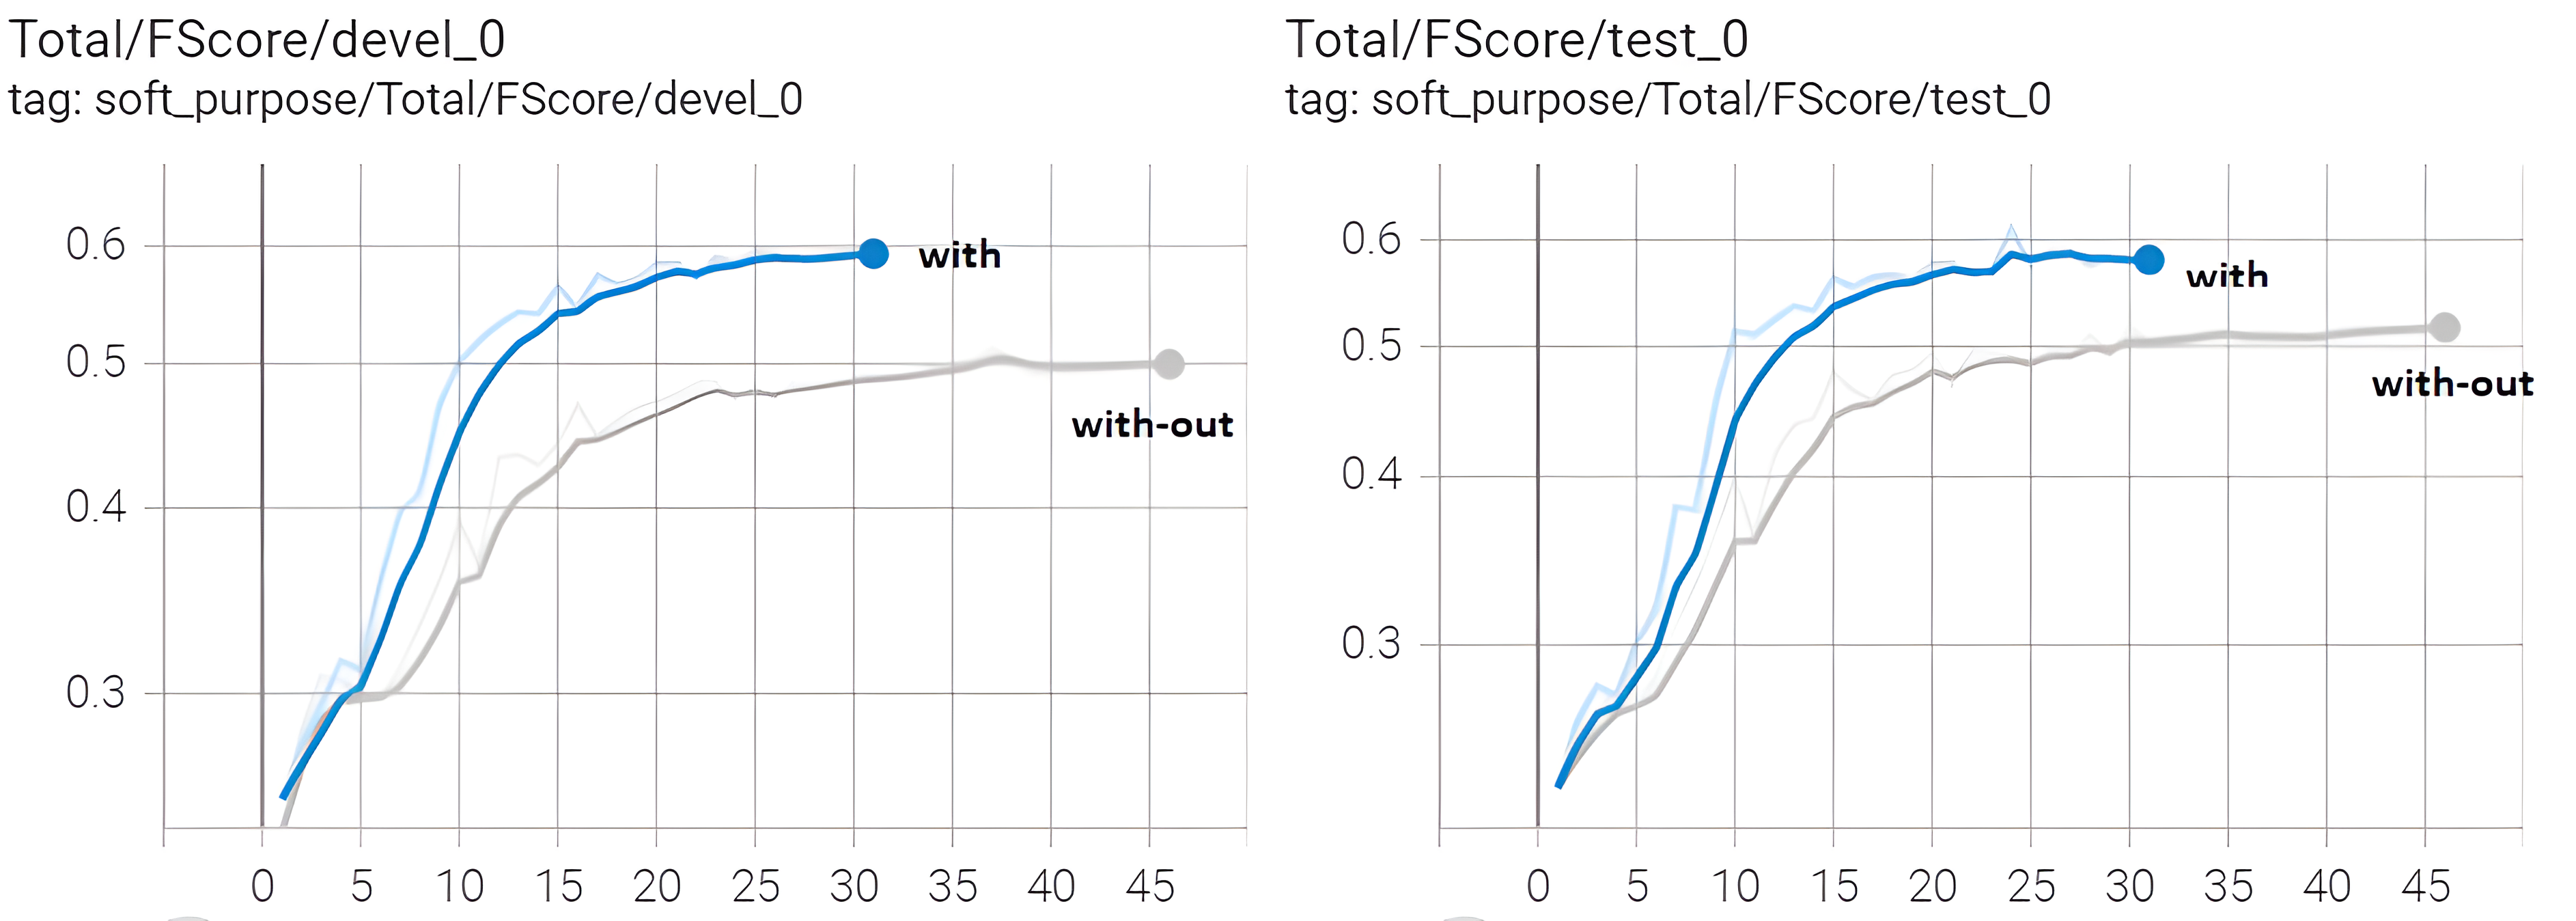
\includegraphics[width=.86\textwidth]{4.graphics/figures/ch_6/1.with_sent_vs_without/HD/Total_Fscore_software_purpose}
	\caption{Software purpose classification (Total) F1-score degrades for devel. set (left) and test set (right) when \emph{Creation/PLoS} sentences are included in the training dataset.}
	\label{fig:chapter06:with}
\end{figure}


\begin{table}[ht]
	\centering
	\caption{Evaluation of software purpose classifier's performance with(+) and without(-) \emph{Creation/PLoS}sentences in the training data set.}
	\begin{tabular*}{0.75\textwidth}{@{\extracolsep{\fill}}  l  l l  l l l } %l left align , c- center
		\hline
		Software Purpose & Metric & Dev+        & Dev-     & Test+  &Test- \\
		\hline 
		Analysis         & F     & 0.64        & 0.71     &0.65     &0.69   \\
		                 & P     & 0.61        & 0.71     &0.60     &0.66   \\
		                 & R     & 0.68        & 0.71     &0.72     &0.73   \\
		\hline
		Data-Collection  & F     & 0.26        &  0.32    & 0.26    & 0.34  \\
					     & P     & 0.25        &  0.33    & 0.22    & 0.30  \\
						 & R     & 0.28        &  0.31    & 0.30    & 0.31  \\		
		
		\hline
		Pre-Processing   & F     & 0.41        &  0.45    & 0.49    & 0.57  \\
						 & P     & 0.36        &  0.37    & 0.45    & 0.49  \\
						 & R     & 0.48        &  0.56    & 0.58    & 0.67  \\
		\hline
		Modeling         & F     & 0.25        &  0.54    & 0.30    & 0.44  \\
					     & P     & 0.27        &  0.54    & 0.28    & 0.42  \\
						 & R     & 0.24        &  0.55    & 0.30    & 0.46  \\
	
		\hline
		Programming      & F     & 0.27        &  0.42    & 0.23    & 0.42  \\
						 & P     & 0.28        &  0.34    & 0.24    & 0.36  \\
						 & R     & 0.27        &  0.55    & 0.23    & 0.51  \\
		
		\hline
		Simulation      & F     & 0.00        &  0.38    & 0.00    & 0.00 \\
						& P     & 0.00        &  0.88    & 0.00    & 0.00  \\
						& R     & 0.00        &  0.25    & 0.00    & 0.00  \\
		
		\hline
		Stimulation     & F     & 0.46        &  0.59    & 0.24    & 0.26 \\
						& P     & 0.40        &  0.76    & 0.21    & 0.24  \\
						& R     & 0.48        &  0.45    & 0.28    & 0.22  \\
		
		\hline
		Visualization   & F     & 0.48        &  0.59    & 0.52    & 0.58  \\
						& P     & 0.46        &  0.59    & 0.46    & 0.54  \\
						& R     & 0.51        &  0.61    & 0.56    & 0.62  \\
		\hline
		Total (software Purpose)	& F     & 0.27        &  0.58*    & 0.30    & 0.54*  \\
								& P     & 0.26        &  0.62*    & 0.26    & 0.56*  \\
								& R     & 0.31        &  0.55*    & 0.32    & 0.65*  \\
		\hline
		Total (software) 	& F     &  0.86*       & 0.84     & 0.83    & 0.83  \\
						& P     &  0.83*       & 0.82     & 0.77    & 0.79*  \\
						& R     &  0.90*       & 0.86     & 0.90*    & 0.87  \\
		\hline
	\end{tabular*}
\end{table}%

Software purpose classifier's performance when trained with \emph{creation/PLoS} sentences versus  without is summarized on the table 6.1. \\

Overall, as indicated in table 6.1, it is observed that including a data set that lacks software purpose annotation harms classifier model’s performance. Since the main goal of this project is to maximize software usage purpose classifer’s performance, for subsequent steps of analysis, the software usage purpose classifier has been trained only with datasets of \emph{PLoS-methods} and \emph{PubMed-full text} by excluding \emph{Creation/PLoS} sentences. 


\section{The impact of larger context}
\label{sec:chapter06:context}

Scientific papers like any other well written documents, have a sequential structure that form abstraction at various levels such as sentence, paragraphs, sections, chapters, etc. These levels of abstractions often determine the meaning of words because each level of abstraction or context conveys a valuable information \citep{ghosh2016contextual}. \\

Likewise, contextual information helps to determine the correct purpose of use of a software. Therefore for each sentence in a text of scientific articles of training data set, various range of neighboring sentences have been incorporated to provide a contextual information. Typically 2 adjacent sentences before a sentence, after a sentence, and before \& after a sentence have been considered. Further more, a context as broad as the whole paragraph has also been considered. \\

Excerpt of the python code for reading neighboring sentences for context has been listed on the \emph{appendix E}. The complete code has been listed on git-hub inside a methods that reads a file\footnote{\url{https://github.com/BeTKH/SoMeNLP/blob/contxt2Sentcs_wo/somenlp/NER/data_handler.py}}. \\

Evaluation of a classifier model with a broader context of two adjacent sentences, improved software purpose classification F-score as shown on the figure 6.3 below. 

\begin{figure}[htbp]
	\centering
	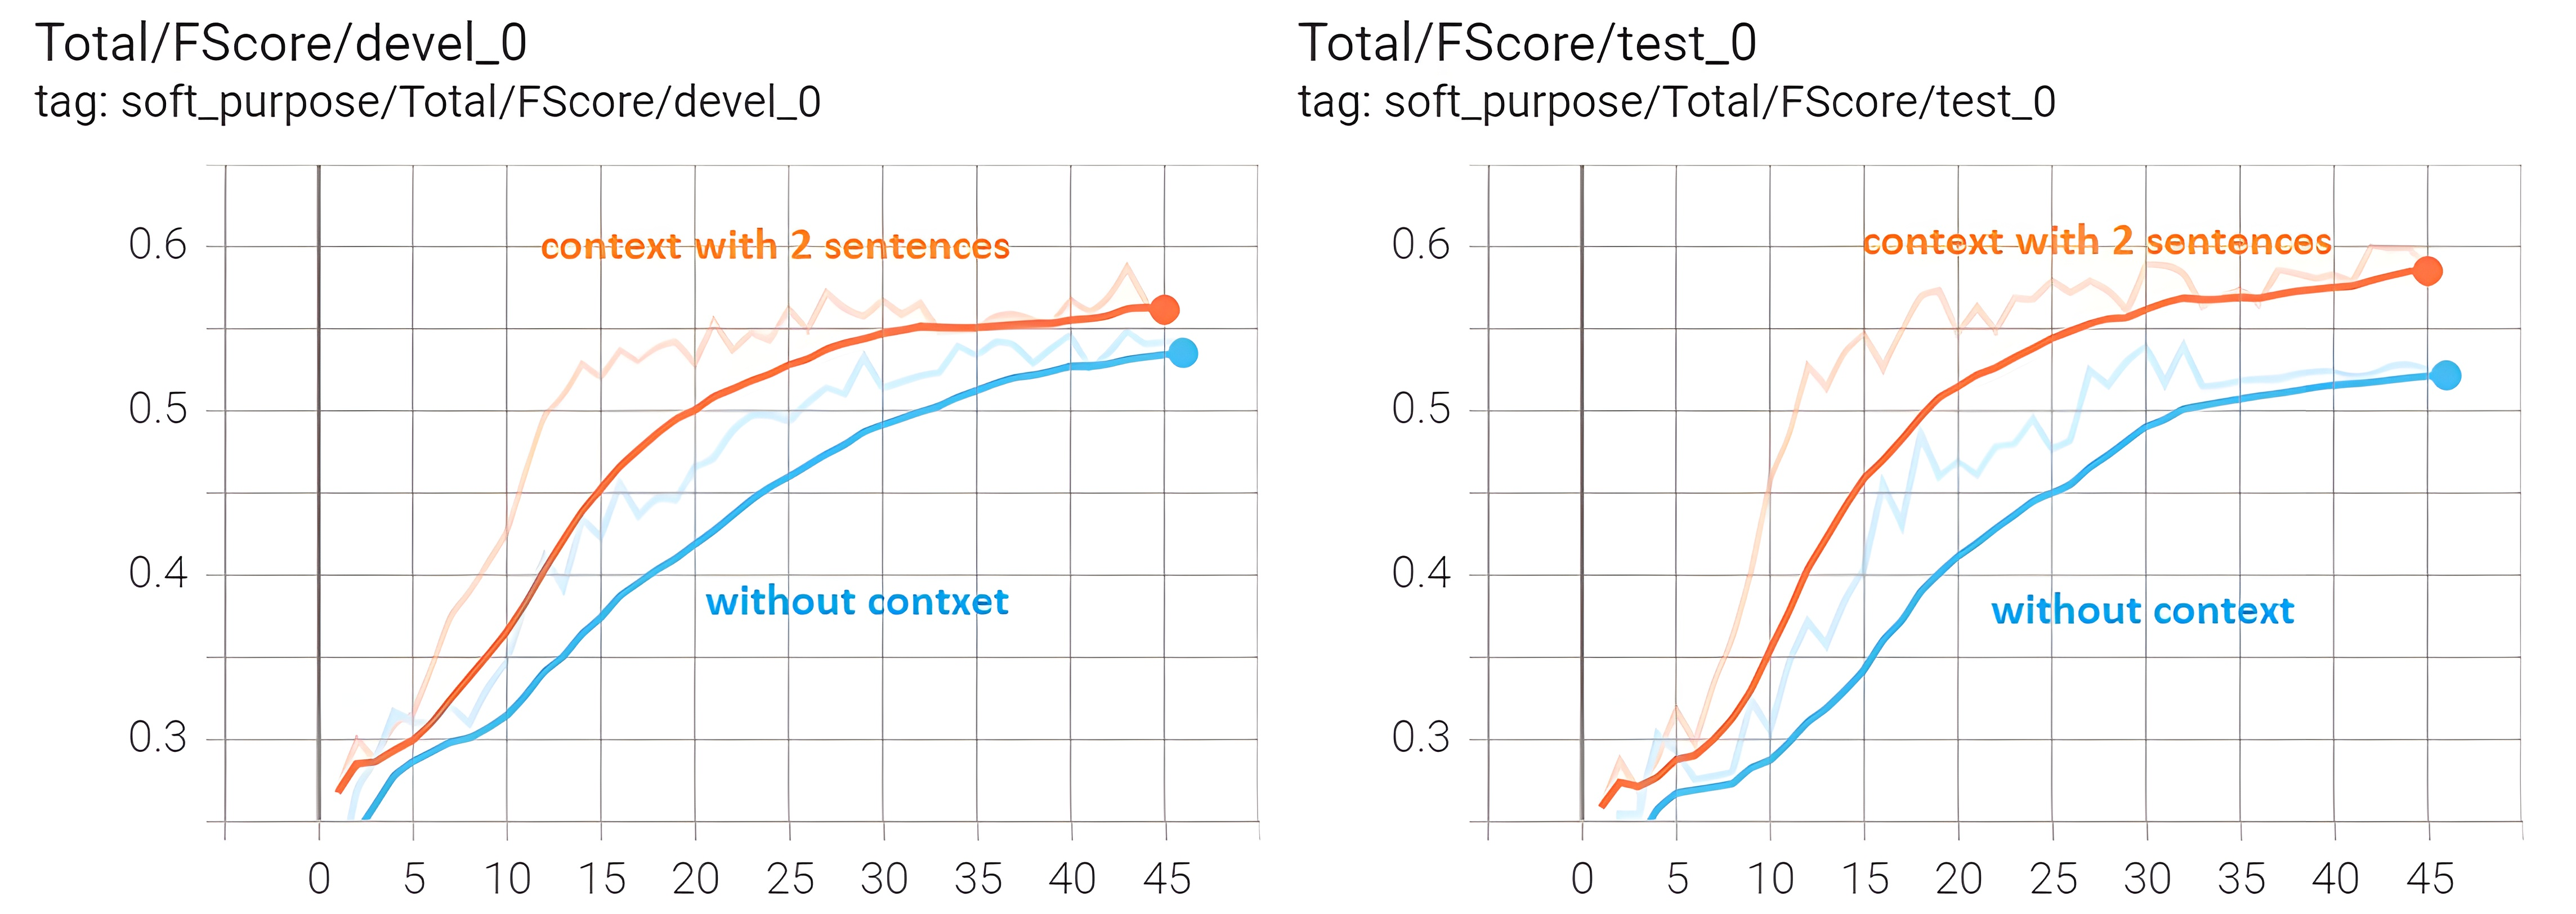
\includegraphics[width=.86\textwidth]{4.graphics/figures/ch_6/2.left_context_vs_right/HD/braoderContextFscore}
	\caption{Software purpose classification (Total) F1-score improves for devel. set (left) and test set (right) when trained with a broader context of two adjacent sentences compared to without context (blue).}
	\label{fig:chapter06:with}
\end{figure}

\subsection{Left vs Right Context within a paragraph}
\label{sec:chapter06:leftvsright}

In addition to a broader context, it was also desired to determine which part of context, left versus right, information is more important for the software purpose classification. Left context refers to sentences prior to a given sentence with in  a paragraph and right context refers to sentences that lie right after a given sentence. To determine the impact of neighboring context on the classifier model's performance, two adjacent sentences from the left and right has been used to train the model separately.  \\

According to the classifier's F1-Score performance, s sentences from the left context information is more important than the right side 2 sentences for context. In addition, the left context (2,0 - sentences) has more significance over both left-and-right context (2,2) sentences. This indicates that the classifier is not benefited any more by including the right context or both contexts as portrayed on the figure 6.4. below. 

\begin{figure}[htbp]
	\centering
	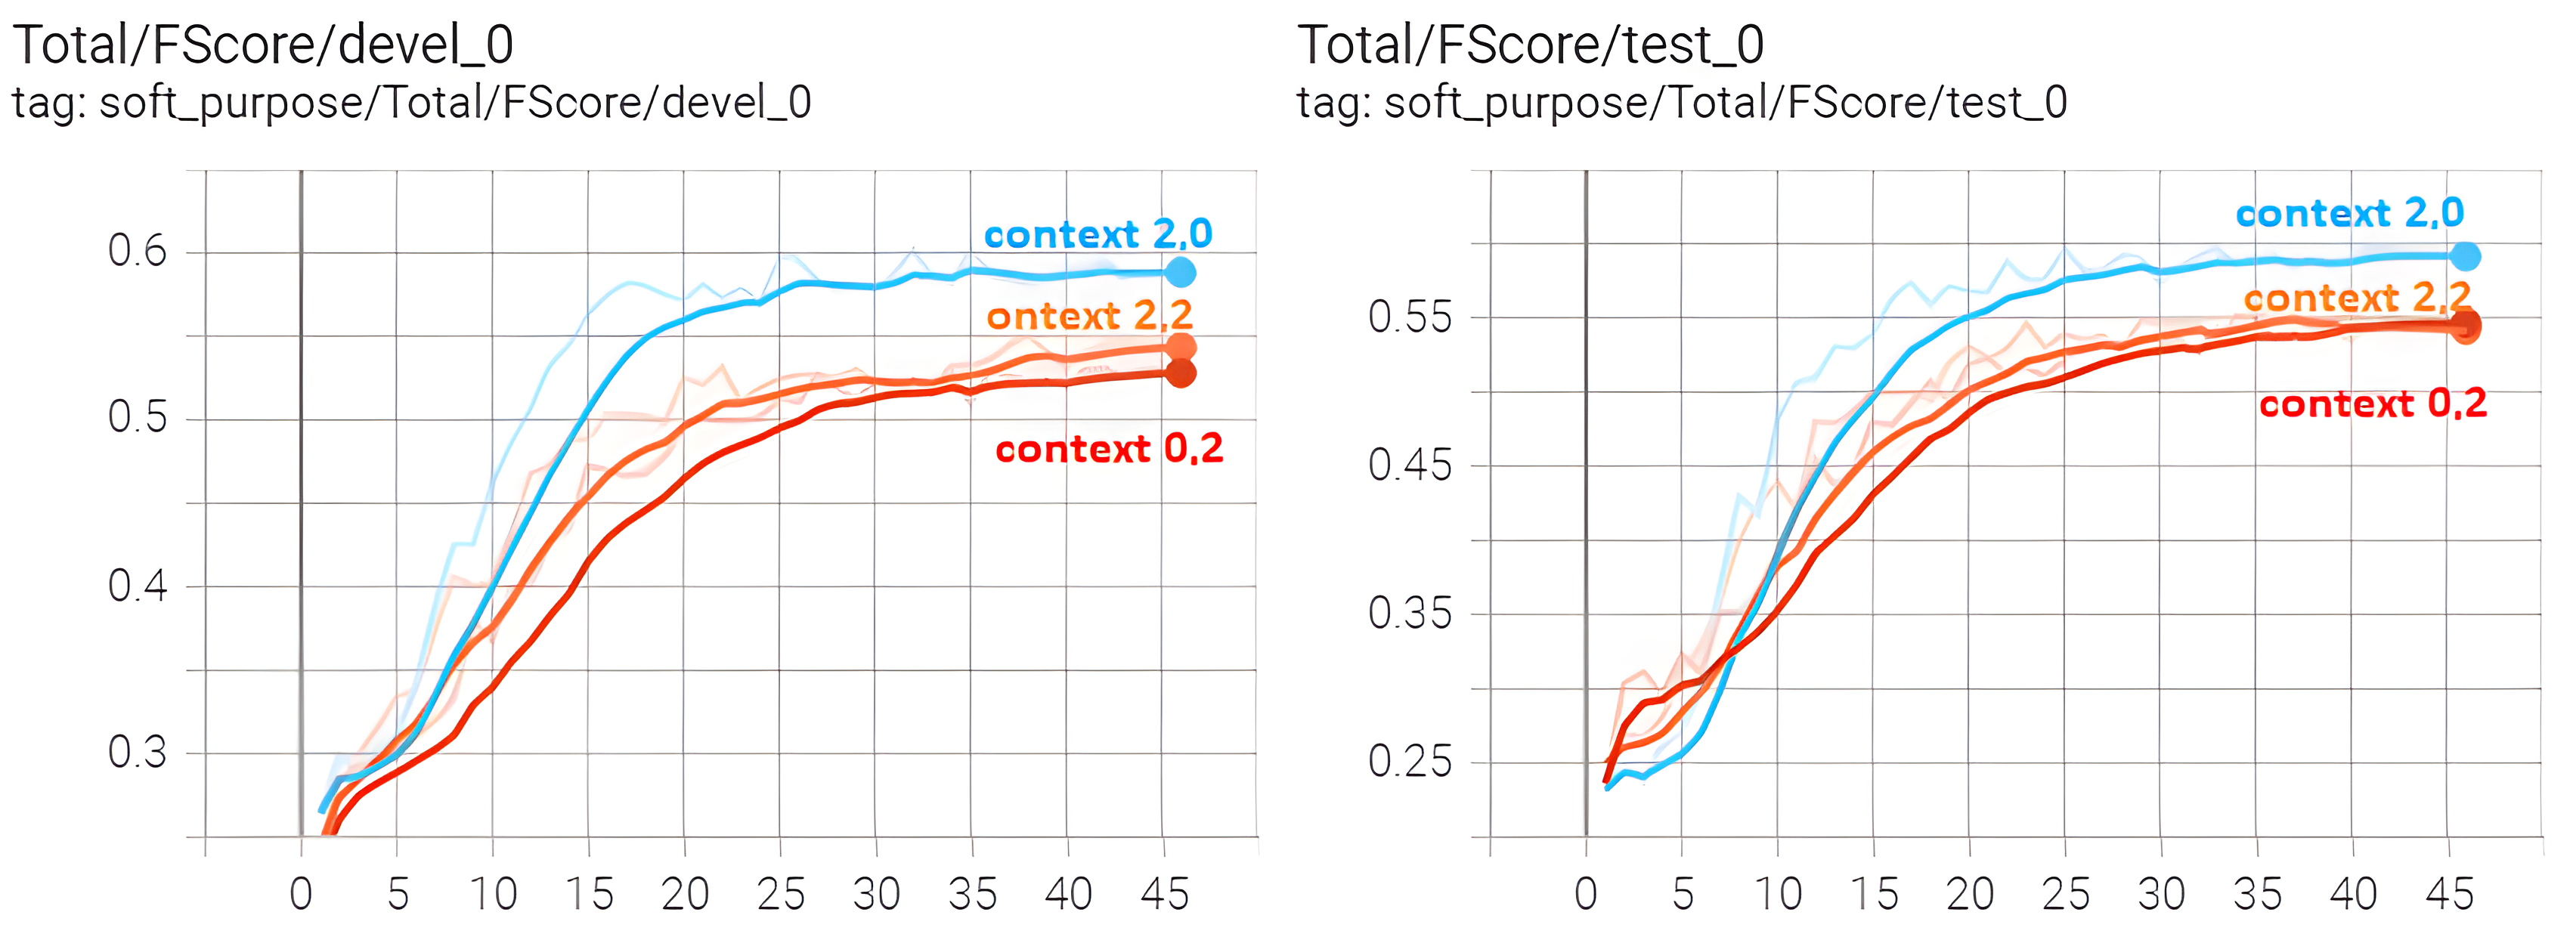
\includegraphics[width=.86\textwidth]{4.graphics/figures/ch_6/2.left_context_vs_right/HD/left_both_right_hd}
	\caption{Software purpose classification (Total) F1-score performance for devel. set (left) and test set (right) when trained with left-context (2,0) has superior performance over right-context (0,2) as well as combined left-and-right-context (2,2).}
	\label{fig:chapter06:with}
\end{figure}


\subsection{Context as whole paragraph}
\label{sec:chapter06:paragraph}

In a common sense, consideration of broader context, such as more than two adjacent sentences, is supposed to improve the classifier’s performance. However, the result of the analysis as indicated on the figure 6.4 reveals that a larger context such as 2 sentences from the left and the right actually yields less F-score performance for the classifier model. To further validate this result, a context as large as whole paragraph has been considered. \\

According to the F-score, software purpose classification actually worsened when an entire sentences in the paragraph is considered as a context information. \\

\begin{figure}[htbp]
	\centering
	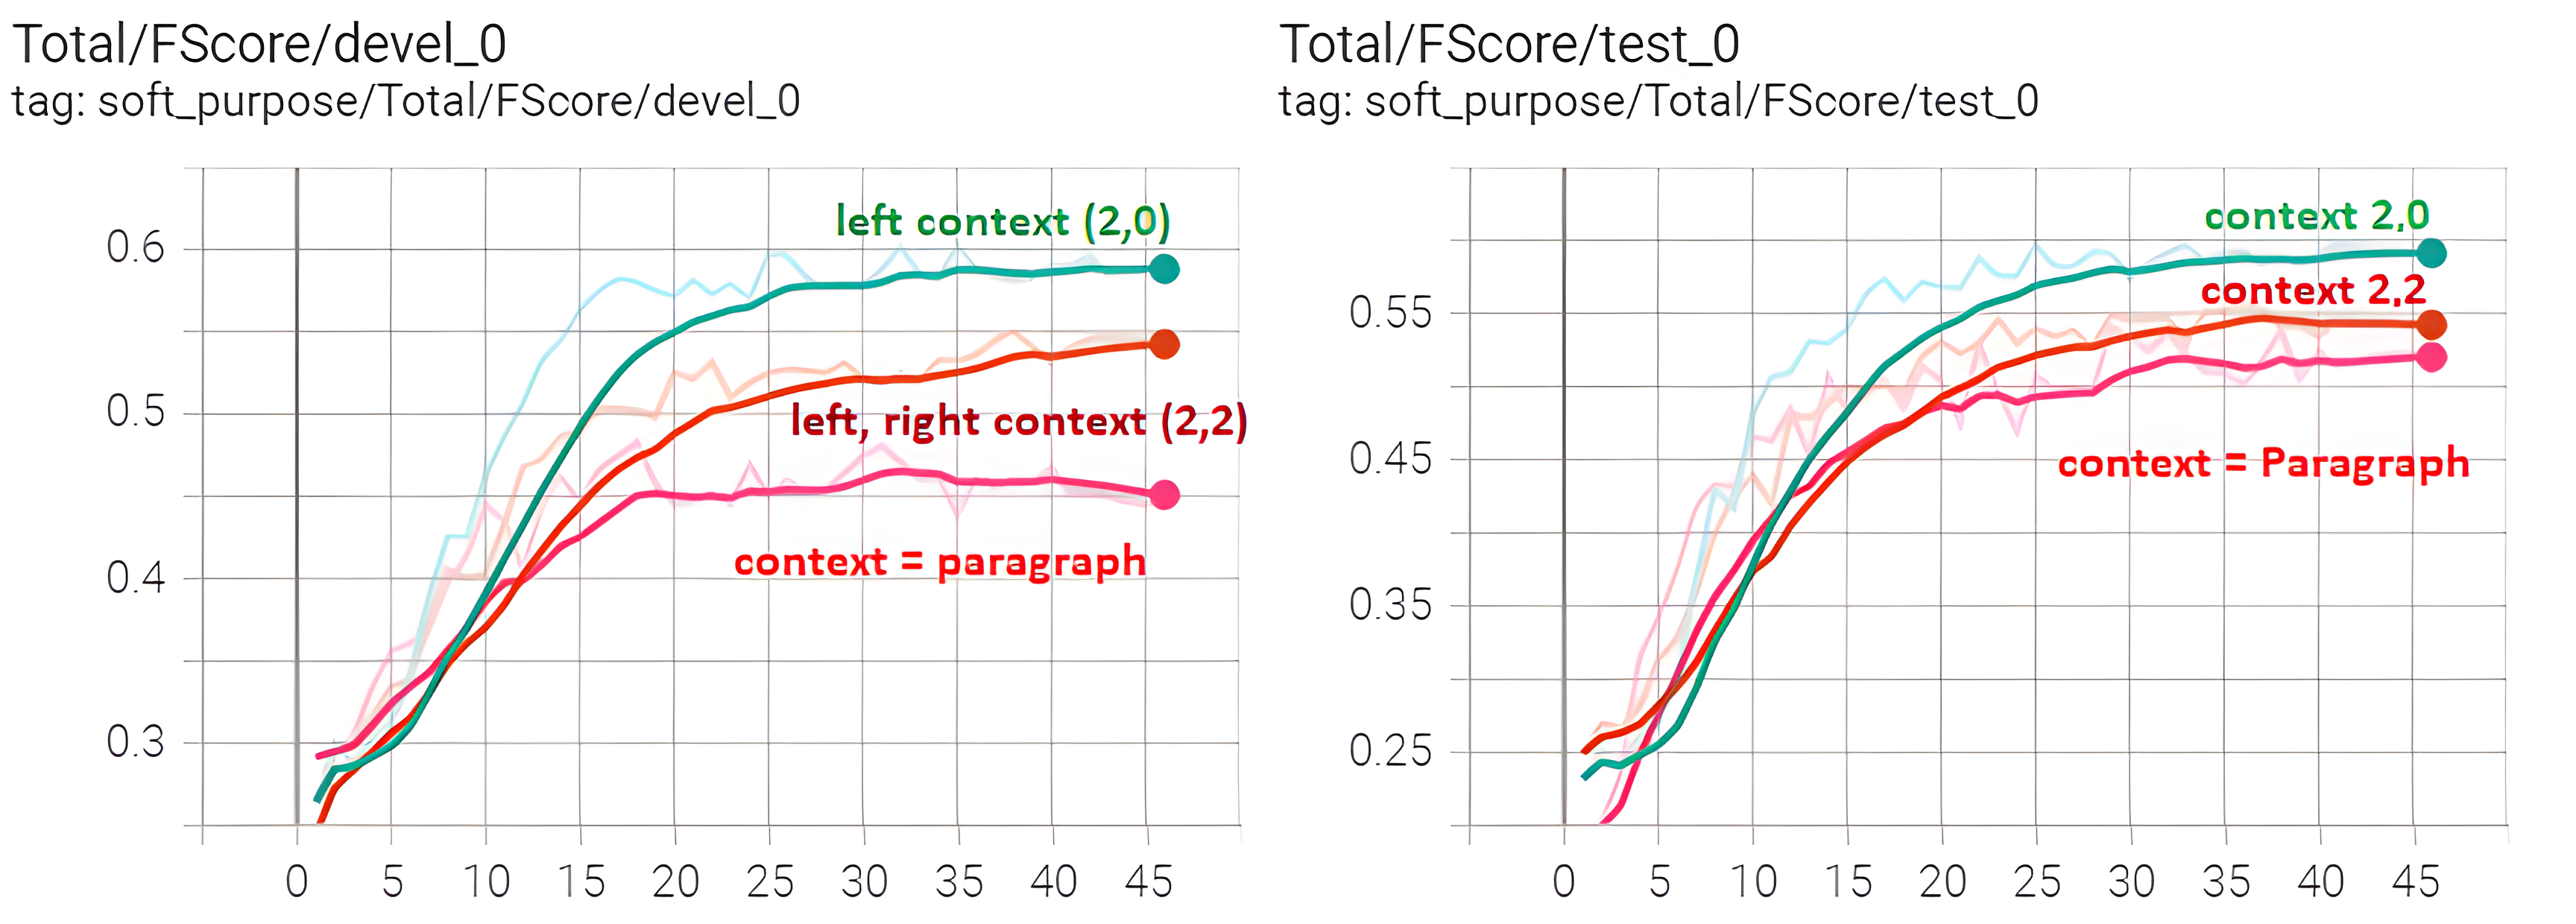
\includegraphics[width=.80\textwidth]{4.graphics/figures/ch_6/2.left_context_vs_right/HD/context_paragrapgh}
	\caption{Software purpose classification (Total) F1-score performance for devel. set (left) and test set (right) deteriorates when very large context, paragraph, is considered.}
	\label{fig:chapter06:with}
\end{figure}


\subsection{Context Outside a Paragraph}
\label{sec:chapter06:contxtOutside}


The other scenario considered was evaluation of software purpose classifier's performance when context is not limited within a paragraph. Accordingly, 2 adjacent sentences for context has been considered within a paragraph versus regardless of paragraph. \\

Evaluation of the classifier's performance indicate that, classifier’s F-score degraded when a context is not limited within a paragraph as shown on the figure 6.6. This agrees with the fact that each paragraph of a scientific publication conveys a specific information and a contextual information outside a paragraph is not useful for the classifier.  The classifier model which considers context outside a paragraph has been listed on \emph{“contxt\_out\_parg”} git-hub branch of SoMeNLP project\footnote{\url{https://github.com/BeTKH/SoMeNLP/tree/contxt_out_parg}}. \\

\begin{figure}[htbp]
	\centering
	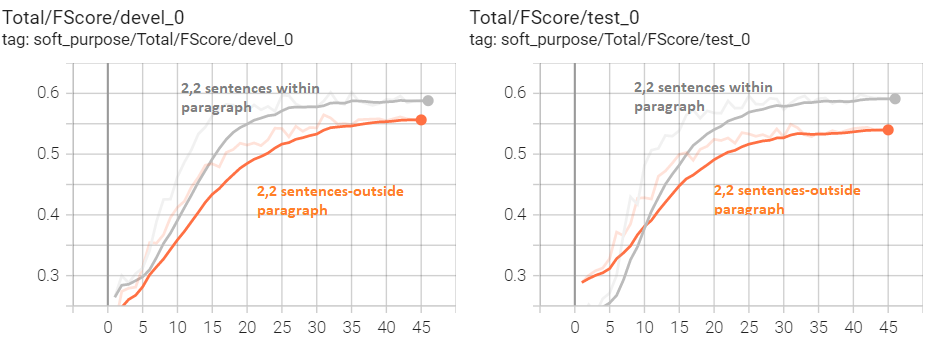
\includegraphics[width=.80\textwidth]{4.graphics/figures/ch_6/2.left_context_vs_right/HD/Fscore_outside_paragrapgh_vs_inside}
	\caption{Software purpose classification (Total) F1-score performance for devel. set (left) and test set (right) did not benefit from context outside a paragraph. }
	\label{fig:chapter06:with}
\end{figure}


Based on evaluation of software purpose classifier's performance, overall it was observed that left context is more important than the right context. In addition, it was observed that context from both left and right as well as a broader context outside a paragraph did not contribute to the classifier's performance in terms of F-score. \\

Based on results,shown on figure 6.6, for all subsequent steps of classifier's evaluation, only two adjacent sentences from the left context have been considered. \\


\section{Classification with 2-Cascade}
\label{sec:chapter06:2lc}

A 4-cascade of multi-class classifier \ac{Sci-BERT} model, shown on the figure 5.6, has been used for the software purpose classification until this point. This model, not only classifies software usage purposes but also other information about software such as software as an application, software types, and mention-types. \\


Overall the 4-cascade \ac{Sci-BERT} multi-class classifier’s performance has been poor regardless of consideration of various factors discussed above. For this reason, it was desired to study weather the removal of intermediate classifier modules would improve software purpose classification or not. Consequently, software-type classifier module and mention-type classifier module, has been removed and the resulting 2-cascade multi-classifier module is shown on the figure 6.7. The software-entity classifier module, however, is kept because identification of software would assist software purpose classification.  \\

\begin{figure}[htbp]
	\centering
	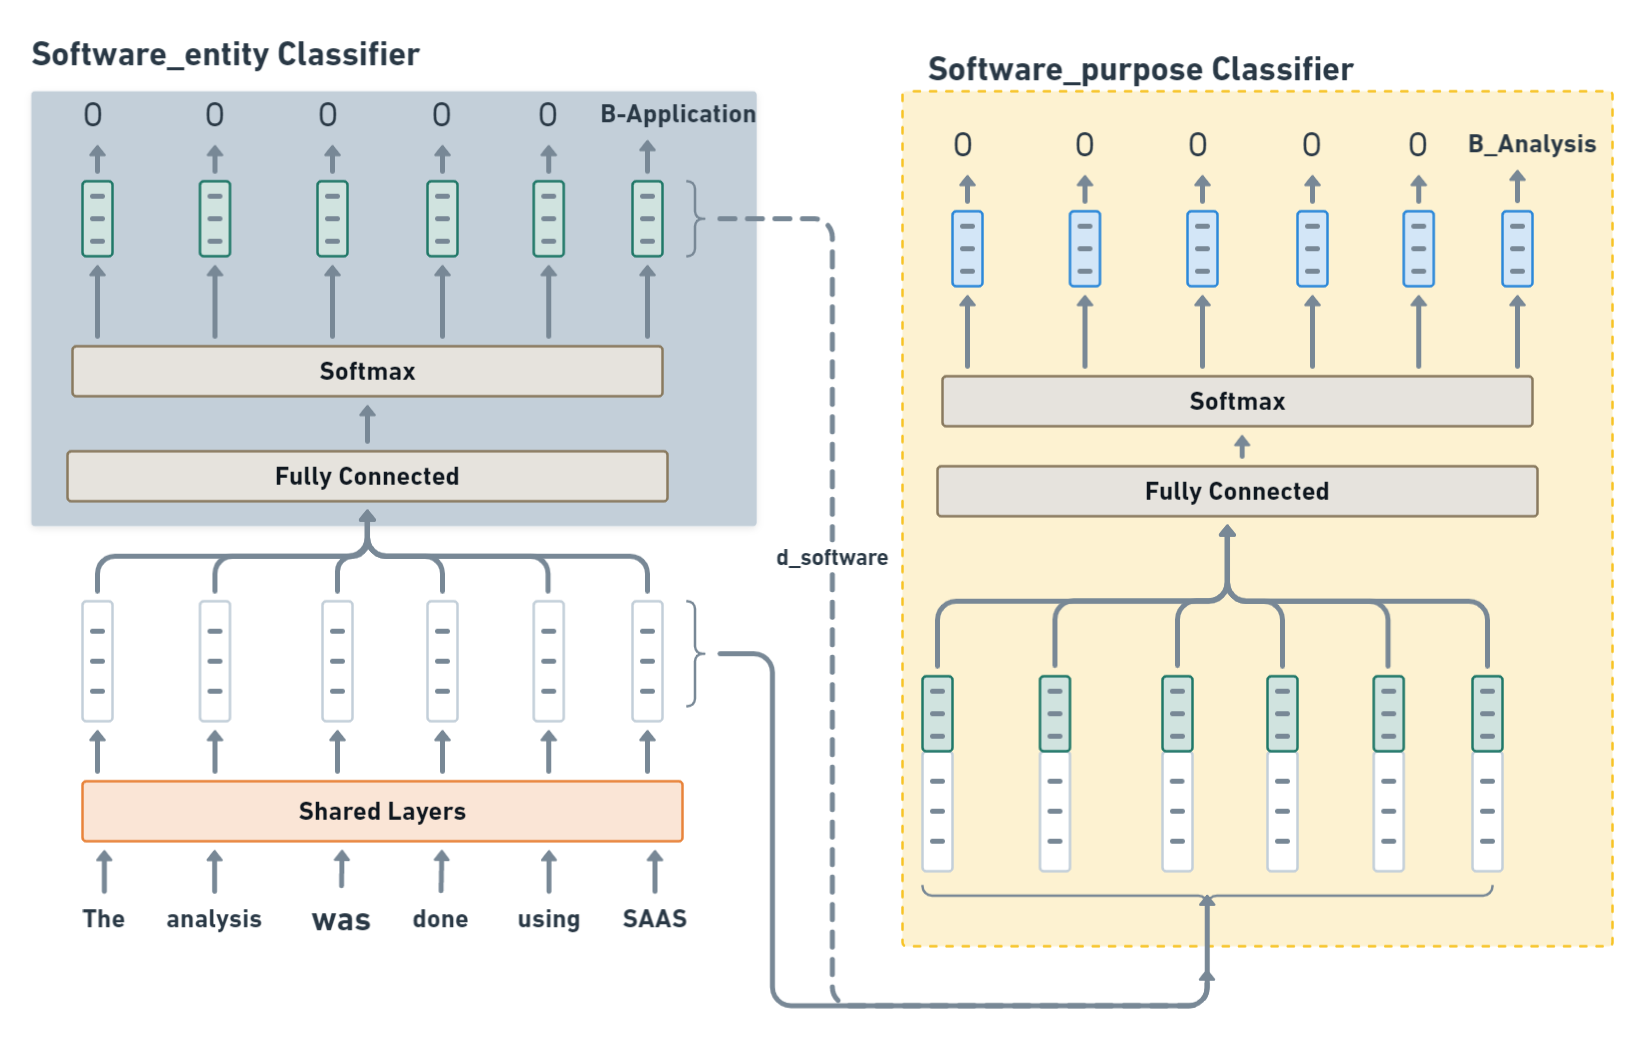
\includegraphics[width=.65\textwidth]{4.graphics/figures/ch_5/2LC}
	\caption{Fully connected, 2-cascade software and software purpose classifier model.}
	\label{fig:chapter06:with}
\end{figure}

Evaluation of the 2-cascade classifier model reveals that overall \emph{software purpose} classification F-score performance has shown small improvement compared to the original 4-cascade classifier module  \ac{Sci-BERT} model, where as the \emph{software classifier’s} performance does not indicate any performance improvement as shown in figures 6.8 and 6.9 respectively.  \\

\begin{figure}[htbp]
	\centering
	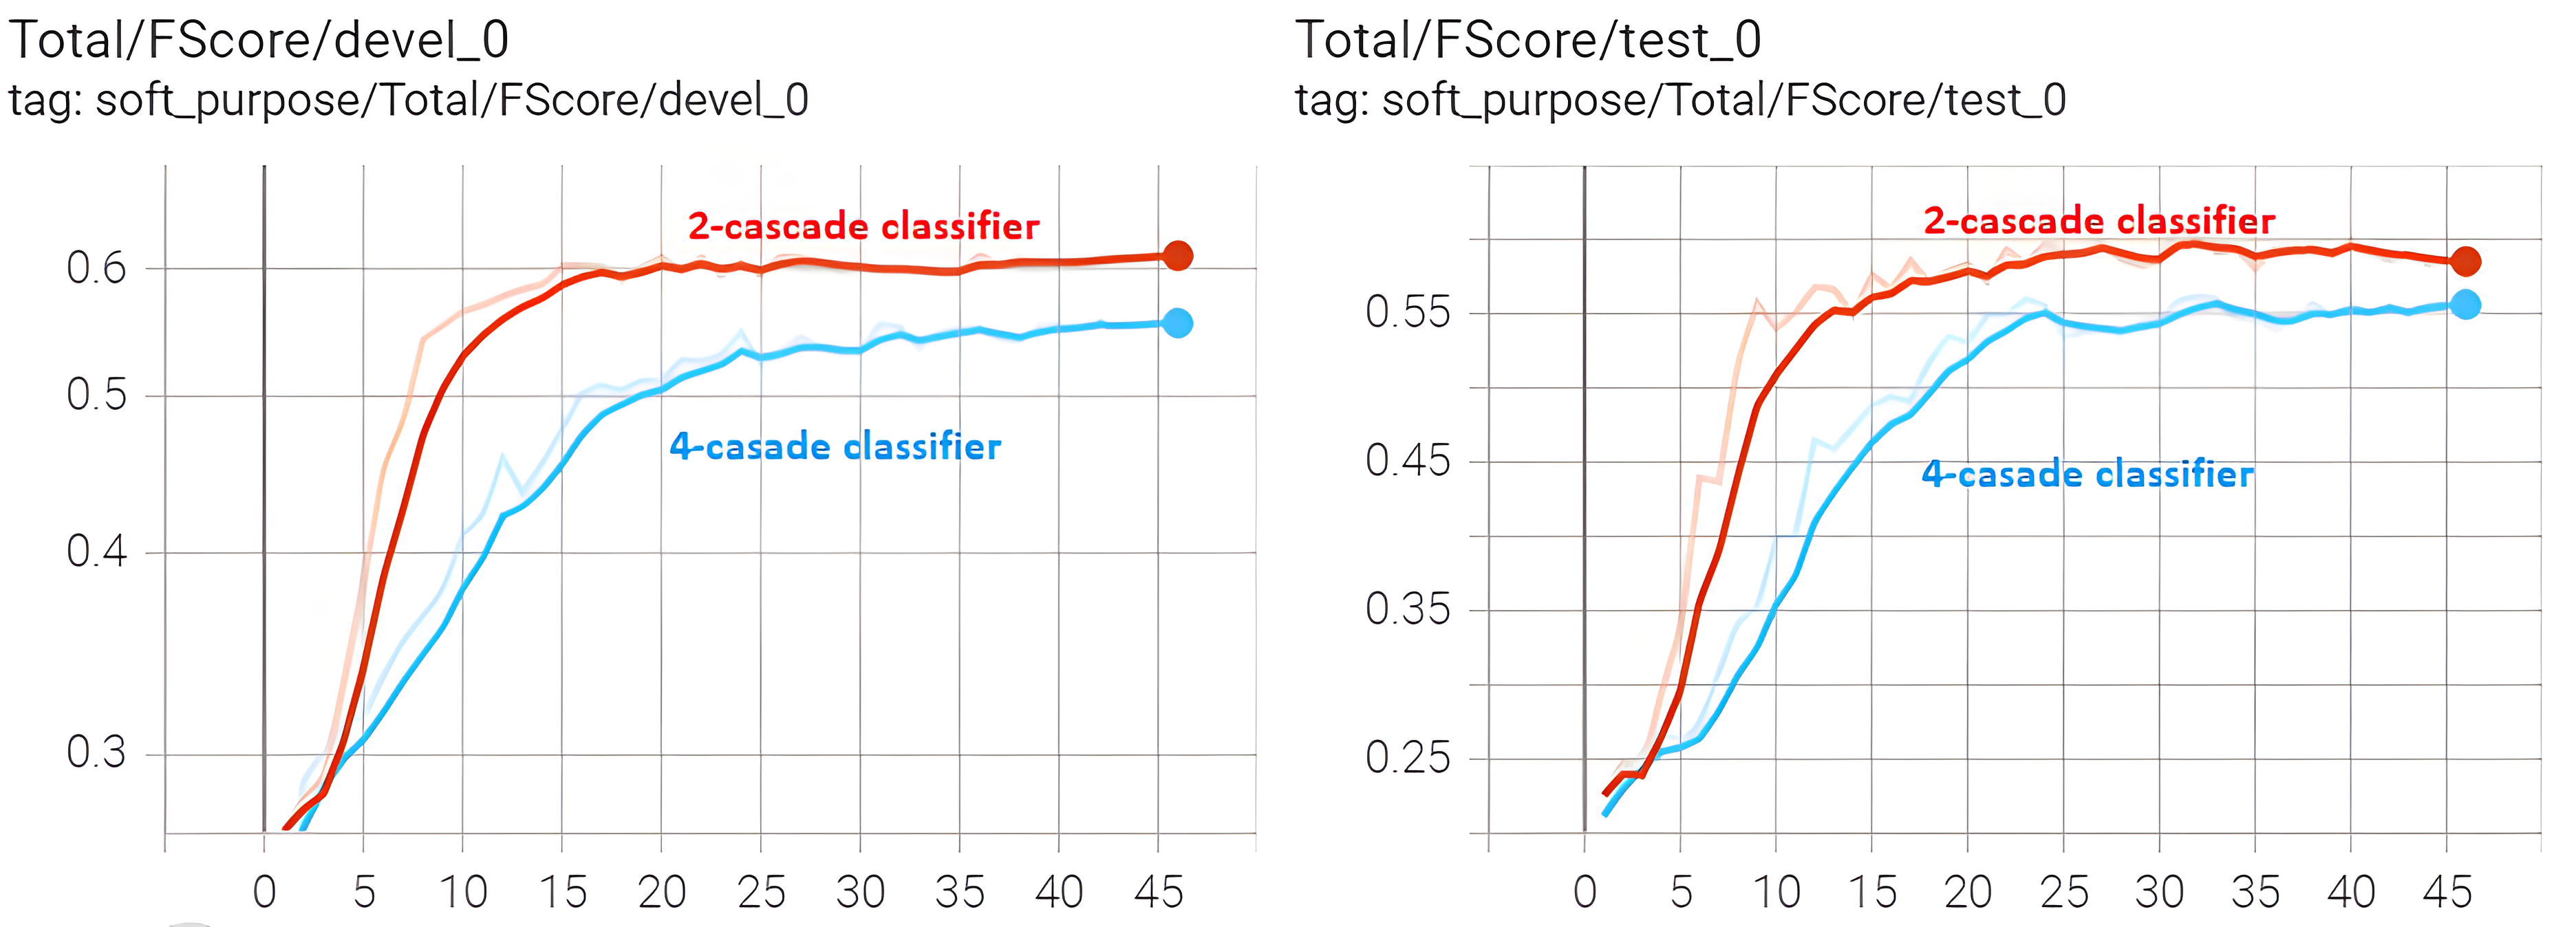
\includegraphics[width=1\textwidth]{4.graphics/figures/ch_6/5.2layerClassifier/HD/4casadeVs2cascade}
	\caption{2-cascade classifier has slightly better (Total) F-score over devl. set(left) and test set(right) for software \emph{purpose classification}.}
	\label{fig:chapter06:with}
\end{figure}


\begin{figure}[htbp]
	\centering
	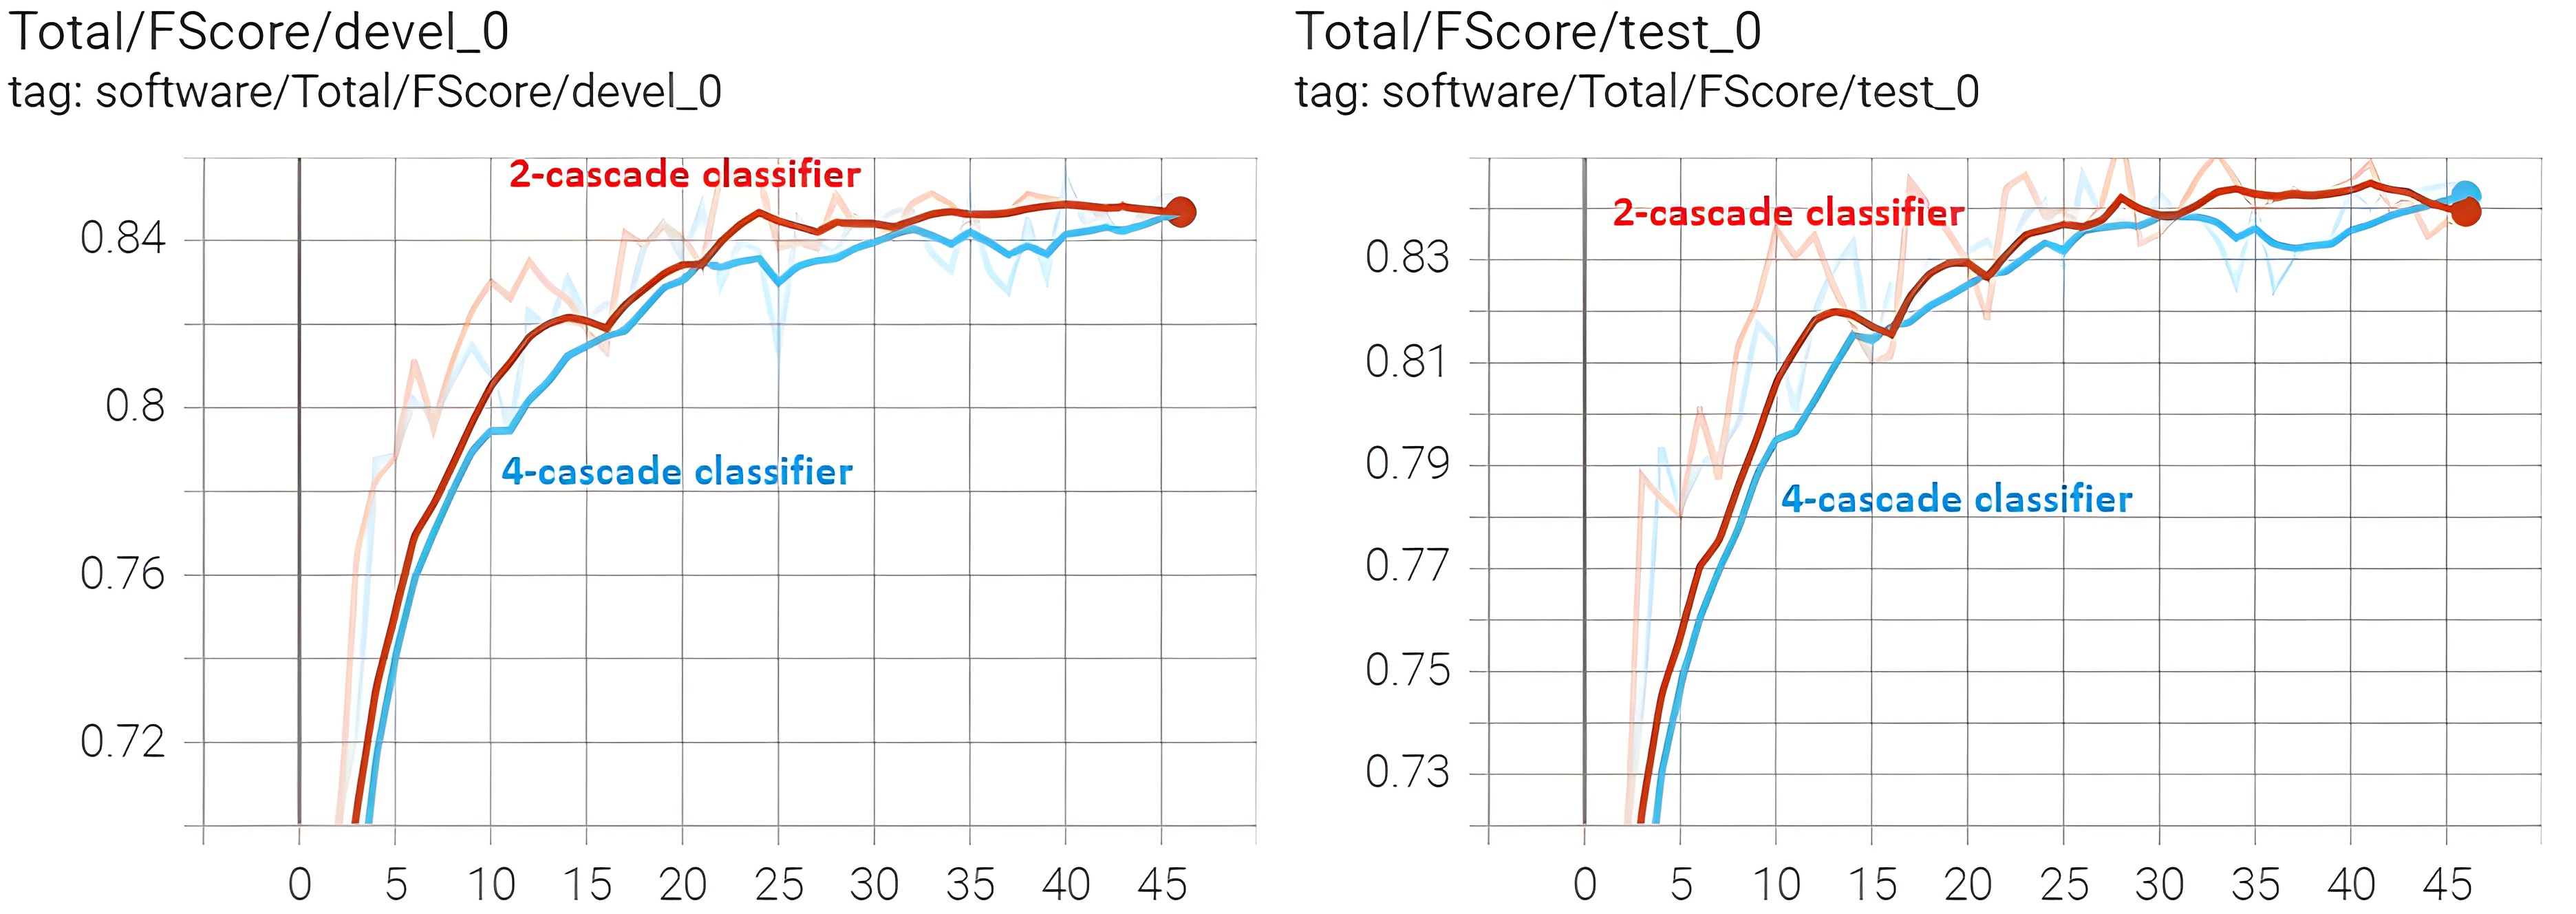
\includegraphics[width=1\textwidth]{4.graphics/figures/ch_6/5.2layerClassifier/HD/4casadeVs2cascade_software}
	\caption{2-cascade classifier has no significant performance improvement in terms of (Total) F-score over devl. set(left) and test set(right) for \emph{software classification}.}
	\label{fig:chapter06:with}
\end{figure}

The evaluation of classifier’s performance by removing the intermediate classifier modules from the 4-cascade model gives a marginal improvement for \emph{software purpose} classification, but not for \emph{software} classification. This might point out, probably flawed classifications of intermediate layers might have an impact on the software purpose classifier which lies at the end of the classification cascade. \\

Since a 2-cascade classifier model has slightly better performance, for the next steps only 2-cascade classifier model has been considered. \\

\section{Bio-BERT vs Sci-BERT}
\label{sec:chapter06:biosci}

As mentioned before, on section 5.3.1, the other variant of BERT model which is trained with SoMeSci dataset in this thesis is Sci-BERT. Even though both \ac{Bio-BERT} and \ac{Sci-BERT} give a contextualized representation of a word in a sentence, representations of a word would differ due to the inherent difference of corpora used for pre-trained models of Bio-BERT and Sci-BERT \citep{beltagy2019scibert,li2019fine}. For this reason, a 2-cascade classifier model has been trained with Bio-BERT and results are compared with Sci-BERT model. \\

Among various varieties of Bio-BERT models, Bio-BERT(base) and Bio-BERT(large) models have bee trained with SoMeSci data set to compare performance with Sci-BERT model. \\

The results of evaluation indicate that  Bio-BERT-large\footnote{\url{https://huggingface.co/dmis-lab/biobert-large-cased-v1.1}} model performed slightly better than the Sci-BERT\footnote{\url{https://huggingface.co/allenai/scibert_scivocab_cased}} model according to the total F-score. However, Sci-BERT has superior performance compared to the Bio-BERT-base\footnote{\url{https://huggingface.co/dmis-lab/biobert-base-cased-v1.2}} model. \\

\begin{figure}[htbp]
	\centering
	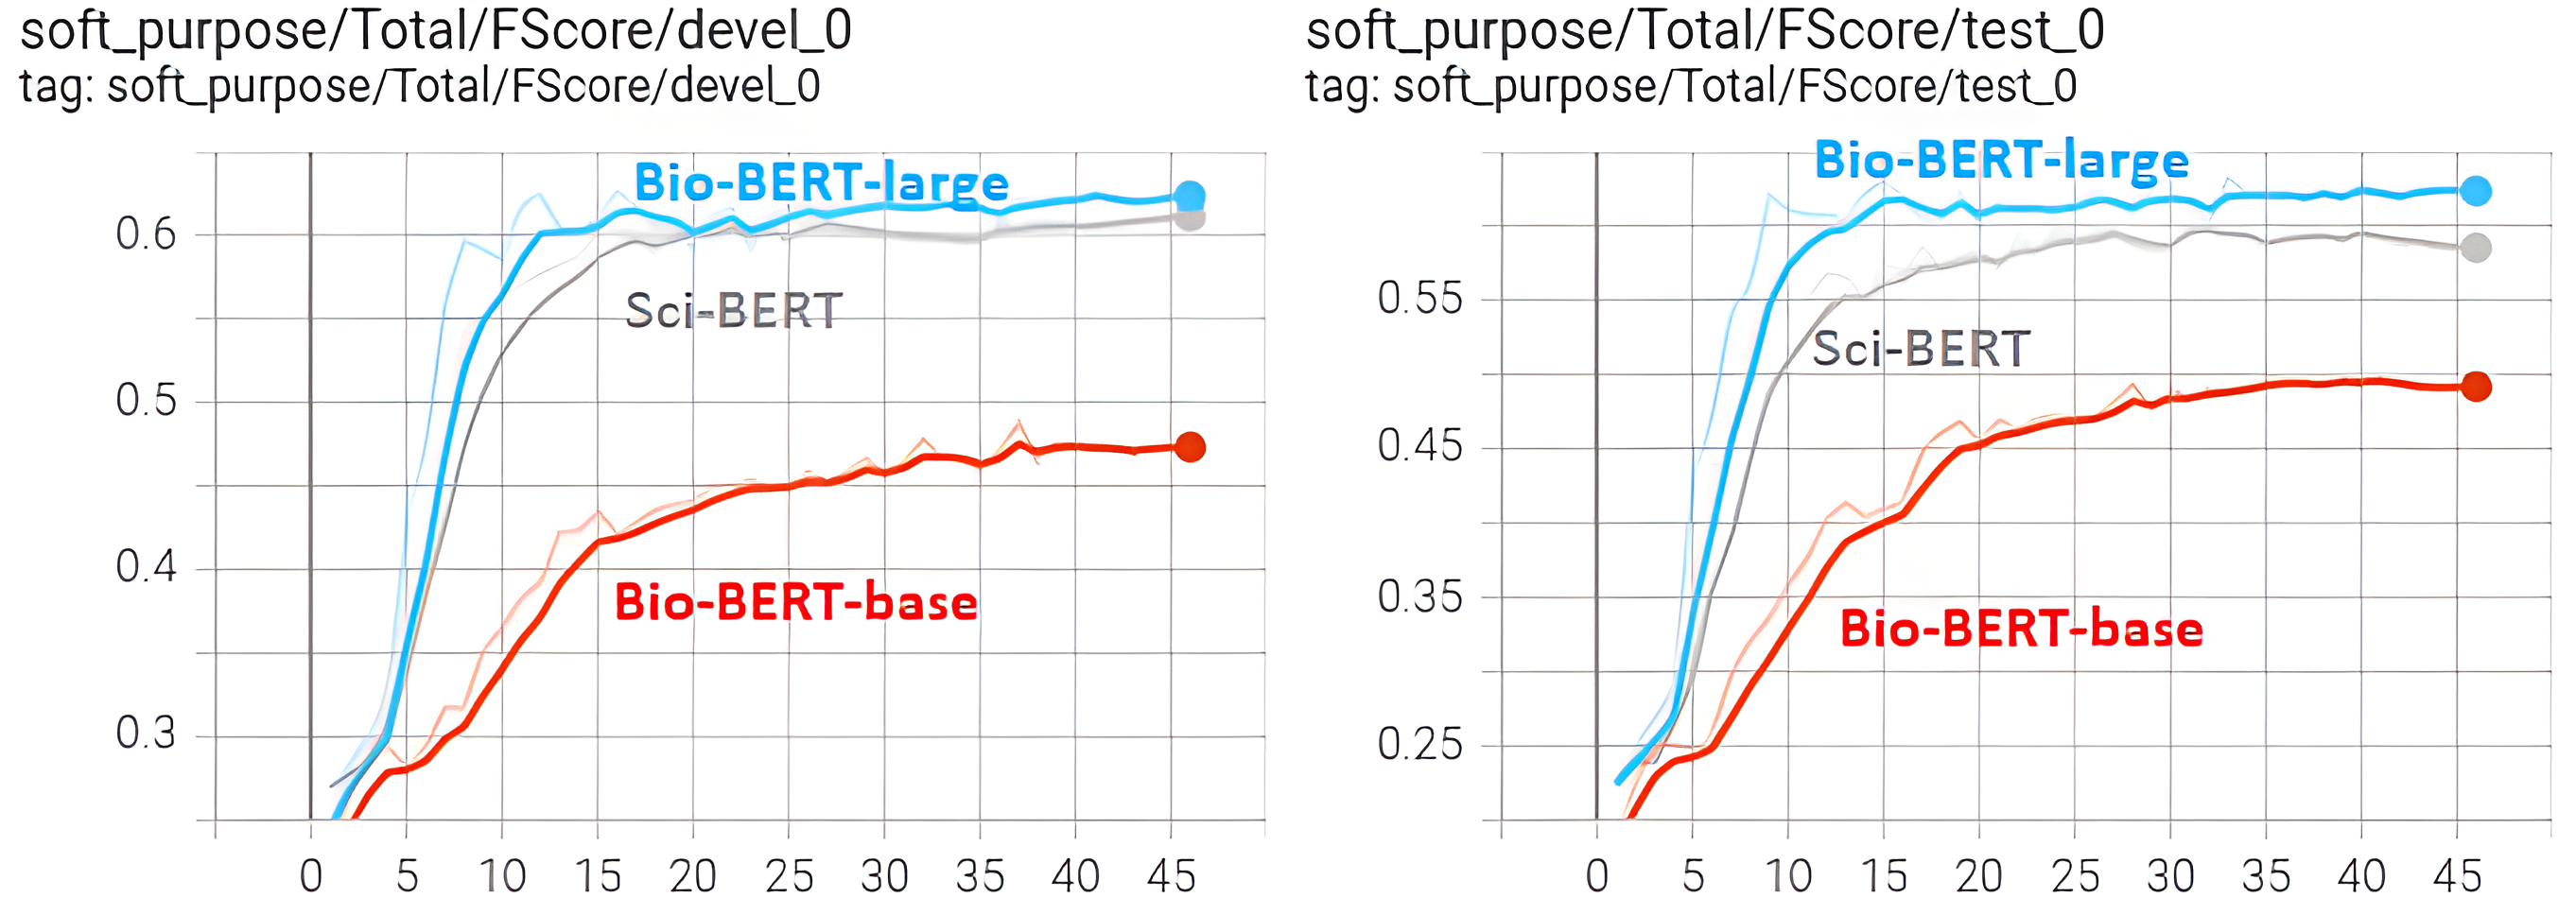
\includegraphics[width=1\textwidth]{4.graphics/figures/ch_6/6.BIoBERT_vs_SCIBERT_2LAYER_Classifier/HD/BIobert-large-small-cybert}
	\caption{2 Cascade \emph{software-purpose} classifier, trained with Bio-BERT-large, Sci-BERT and Bio-BERT-base indicates that the large model of Bio-BERT has superior performance (Total) F-score over Sci-BERT as well as Bio-BERT-base when tested with dev-set(left) and test-set(right).}
	\label{fig:chapter06:with}
\end{figure}






















